\chapter{Finite Difference Method (FDM)}
FDM er en numerisk metode for å løse ODE og PDE ved å diskretisere domenet og tilnærme den deriverte med differanser.

\section{Teori}
\subsection{Taylors formel}
\begin{theorem}{Taylor-rekke for to variabler}{taylor}
	La \(u_m^{n} = u(x_m, t_n) \approx u(x, t)\) være approksimasjonen av den eksakte løsningen \(u\) i punktet \((x_m, t_n)\).
	\begin{align} \label{eq:taylor}
		u_{m+1}^{n+1} &= \sum_{i=0}^{p} \frac{1}{i!} \left(h \partial_x + k \partial_t\right)^i u(x, t) + r_{p+1}(x, t) \tag{taylor} \\
		r_p & = \frac{1}{(p+1)!} \left(h \partial_x + k \partial_t\right)^{p+1} u(x, t) \tag{rest}
	\end{align}
	der \(h, k\) er steglengdene i \((x, t)\) og \(p\) er ordren til Taylor-rekken.
\end{theorem}
\begin{remark*}{Uniform Gridstørrelse}{}
	Hvis vi har en uniform gridstørrelse \(\mathbb{G}\) i \(x\) og \(t\), kan vi skrive:
	\[\mathbb{G} = \{(x_m, t_n) \mid x_m = x_0 + mh, t_n = t_0 + nk \text{ for } m = 0, 1, \ldots, M \text{ og } n = 0, 1, \ldots, N\}\]
	der \(h\) er steglengden i \(x\) og \(k\) er steglengden i \(t\).
\end{remark*}

\section{Motivasjon}
Gitt en vilkårlig differensiallikning (ODE), som f.eks. \( \ddn[f(x)]{2}{x} = f(x) - x^3 \)\label{eq:ode} med randbetingelser: \( f(x_0) = \alpha \) og \( f(x_N) = \beta \).
Denne ODE har allerede en eksakt løsning: \( f(x) = c_0e^x + c_1e^{-x} + x^3 + 6x \)\label{eq:exact}.
Men, hva om vi ikke har en eksakt løsning? Da kan vi bruke FDM til å tilnærme løsningen.

\section{FDM-oppskrift}
\begin{enumerate}
	\item \textbf{Diskretisering:} Del intervallet \(x \in [\alpha, \beta]\) inn i \(N\) like store delintervaller med \(x_i = \alpha + ih\) for \(i = 0,1,\ldots,N\) og \(h = 2/N\)
	\item \textbf{Taylor-utvikling:} Rekkeutvikle \(f(x \pm h)\) rundt \(x\).
	\item \textbf{Differanse metoder:} Finn en lineærkombinasjon av \(f(x \pm h)\) som tilnærmer den deriverte.
	      \begin{align}
		      C_{-1}f(x - h) + C_0f(x) + C_1f(x + h)   & = \ddn[f(x)]{2}{x} + \mathcolor{blue}{O(h)} \tag{Central} \label{eq:center}    \\
		      C_{0}f(x) + C_1f(x + h ) + C_2f(x + 2h)  & = \ddn[f(x)]{2}{x} + \mathcolor{blue}{O(h^2)} \tag{Forward} \label{eq:forward} \\
		      C_{-2}f(x - 2h) + C_{-1}f(x-h) + C_0f(x) & = \ddn[f(x)]{2}{x} + \mathcolor{blue}{O(h)} \tag{Backward} \label{eq:backward}
	      \end{align}
	\item \textbf{Diskretiser og løs ODE:} Anvend en av disse metodene, f.eks. \ref{eq:center} på \ref{eq:ode} og løs ligningssettet \(T_h \vec{f} = \vec{b}\), hvor \(T_h\) er en tri-diagonal.
\end{enumerate}

\section{Differanseoperatorer}

Differanseoperatorer er diskrete tilnærminger av deriverte og kan brukes til å konstruere differanseskjemaer for numerisk løsning av \gls{ode} og \gls{pde}.

Differanseoperatorer er fundamentale byggeklosser for diskretisering av deriverte, og danner grunnlaget for numeriske metoder for differensiallikninger.

\subsection{Fremover differanseoperator}
\begin{definition}{Fremover differanse}{}
	\begin{equation}
		\Delta_h u(x) = u(x + h) - u(x) \label{eq:forward_diff}
	\end{equation}
	der $h > 0$ er steglengden.
\end{definition}

\begin{remark*}{}{}
	Fremover differanse tilnærmer den første deriverte med nøyaktighet $O(h)$:
	\begin{equation}
		\frac{\Delta_h u(x)}{h} = u'(x) + \frac{h}{2}u''(x) + O(h^2)
	\end{equation}
\end{remark*}

\subsection{Bakover differanseoperator}
\begin{definition}{Bakover differanse}{}
	Bakover differanseoperatoren er definert som:
		\begin{align*}
			\nabla_h u(x) & = \frac{1}{h} \left( u(x) - u(x - h) \right) \tag{bakover} \\
			r_1(x) & = \frac{h}{2}u''(x) + O(h^2) \tag{rest}
		\end{align*}
		der \(h > 0\) er steglengden og \(r_p\) er restleddet.
	\end{definition}
\begin{remark*}{}{}
	Bakover differanse tilnærmer også den første deriverte med nøyaktighet $O(h)$, men bruker tidligere punkter:
	\begin{equation}
		\frac{\nabla_h u(x)}{h} = u'(x) - \frac{h}{2}u''(x) + O(h^2)
	\end{equation}
\end{remark*}

\begin{example}{}{}
	\( f''(x) = f(x) - x^3 \) med \( [f(0), f(2)] = [0, 20] \) og \( N = 5 \). Det gir 1D FDM-ligningssettet med sentral differanseoperator:
	\begin{align*}
		\overbrace{
			\begin{bmatrix}
				1             & 0                  & 0             & \cdots & 0             \\
				\frac{1}{h^2} & -\frac{2}{h^2} - 1 & \frac{1}{h^2} & \cdots & 0             \\
				0             & \ddots             & \ddots        & \ddots & \vdots        \\
				\vdots        & \ddots             & \ddots        & \ddots & \frac{1}{h^2} \\
				0             & \cdots             & 0             & 0      & 1
			\end{bmatrix}}^{L_h}
		\overbrace{
			\begin{bmatrix}
				f(x_0) \\ f(x_1) \\ \vdots \\ f(x_{N-1}) \\ f(x_N)
			\end{bmatrix}}^{\vec{f}}
		            & =
		\overbrace{
		\begin{bmatrix}
				\alpha \\ h^2(x_1^3 - x_1) \\ \vdots \\ h^2(x_{N-1}^3 - x_{N-1}) \\ \beta
			\end{bmatrix}}^{\vec{b}} \\
		L_h \vec{f} & = \vec{b}\tag{SUS!}
	\end{align*}

	\vspace{0.5em}

	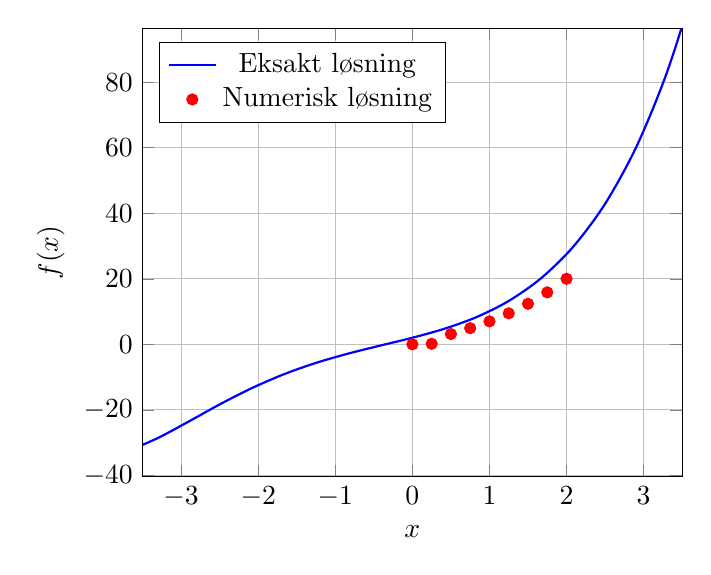
\begin{tikzpicture}
		\begin{axis}[
				xlabel={\(x\)},
				ylabel={\(f(x)\)},
				grid=major,
				legend pos=north west,
				xmin=-3.5,
				xmax=3.5,
				xtick={-3, -2, -1, 0, 1, 2, 3},
			]
			\addplot[smooth, thick, blue] {x^3 + 6*x + exp(x) + exp(-x)};
			\addplot[only marks, red] coordinates {
					(0, 0)
					(0.25, 0.1516)
					(0.5, 3.125)
					(0.75, 4.922)
					(1, 7)
					(1.25, 9.453)
					(1.5, 12.375)
					(1.75, 15.859)
					(2, 20)
				};
			\legend{Eksakt løsning, Numerisk løsning}
		\end{axis}
	\end{tikzpicture}
	\label{fig:ode}
\end{example}

\subsection{Sentral differanseoperator}
\begin{definition}{Sentral differanse}{}
	\begin{equation}
		\delta_h u(x) = u(x + h/2) - u(x - h/2) \label{eq:central_diff}
	\end{equation}
\end{definition}

\begin{remark*}{}{}
	Sentral differanse gir en mer nøyaktig tilnærming av den første deriverte:
	\begin{equation}
		\frac{\delta_h u(x)}{h} = u'(x) + O(h^2)
	\end{equation}
	Dette gjør den til et foretrukket valg når høyere presisjon er nødvendig.
\end{remark*}

\subsection{Andre ordens sentral differanseoperator}
\begin{definition}{Andre ordens sentral differanse}{}
	\begin{equation}
		\delta_h^2 u(x) = u(x + h) - 2u(x) + u(x - h) \label{eq:second_central_diff}
	\end{equation}
\end{definition}

\begin{proposition}{Tilnærming til andre deriverte}{}
	Andre ordens sentral differanseoperator gir en approksimering av den andre deriverte med nøyaktighet $O(h^2)$:
	\begin{equation}
		\frac{\delta_h^2 u(x)}{h^2} = u''(x) + O(h^2)
	\end{equation}
\end{proposition}

\begin{remark*}{}{}
	Denne operatoren er spesielt nyttig for numerisk løsning av elliptiske og parabolske partielle differensiallikninger, som varmeledningslikningen og Poissons likning.
\end{remark*}

\subsection{Gjennomsnittsoperator}
\begin{definition}{Gjennomsnittsoperator}{}
	\begin{equation}
		\mu_h u(x) = \frac{1}{2} \left( u(x + h/2) + u(x - h/2) \right) \label{eq:avg_op}
	\end{equation}
\end{definition}

\begin{remark*}{}{}
	Gjennomsnittsoperatoren kan brukes til å konstruere differanseskjemaer med høyere nøyaktighet ved å kombinere fremover og bakover differanser.
	Den kan også brukes til å lage differanseskjemaer med høyere nøyaktighet ved å kombinere fremover og bakover differanser.
\end{remark*}

\subsection{Skiftoperator}
\begin{definition}{Skiftoperator}{}
	\begin{equation}
		E_h u(x) = u(x + h) \label{eq:shift_op}
	\end{equation}
\end{definition}

\begin{remark*}{}{}
	Skiftoperatoren kan brukes til å uttrykke alle andre differanseoperatorer, for eksempel:
	\begin{align}
		\Delta_h   & = E_h - I           \\
		\nabla_h   & = I - E_{-h}        \\
		\delta_h^2 & = E_h - 2I + E_{-h}
	\end{align}
	der $I$ er identitetsoperatoren, $Iu(x) = u(x)$.
\end{remark*}

\begin{theorem}{Differanseoperatorenes relasjoner}{}
	Differanseoperatorene er relatert til hverandre på følgende måter:
	\begin{align}
		\delta_h^2 & = \Delta_h \nabla_h = \nabla_h \Delta_h \\
		\delta_h   & = \mu_h \Delta_h = \mu_h \nabla_h E_h   \\
		E_h        & = I + \Delta_h
	\end{align}
	der $I$ er identitetsoperatoren, $Iu(x) = u(x)$.
\end{theorem}

\begin{remark*}{}{}
	Fremover- og bakover-differanseoperatorer er asymmetriske og gir første ordens nøyaktighet,
	mens sentral differanse er symmetrisk og gir andre ordens nøyaktighet ved tilnærming av første deriverte.
\end{remark*}

\begin{example}{Anvendelse av differanseoperatorer}{}
	For funksjonen $u(x) = x^2$ ved $x=1$ med $h=0.1$:
	\begin{align*}
		\Delta_h u(1)   & = (1+0.1)^2 - 1^2 = 1.21 - 1 = 0.21                       \\
		\nabla_h u(1)   & = 1^2 - (1-0.1)^2 = 1 - 0.81 = 0.19                       \\
		\delta_h^2 u(1) & = (1+0.1)^2 - 2(1^2) + (1-0.1)^2 = 1.21 - 2 + 0.81 = 0.02
	\end{align*}
	Dette stemmer overens med andre deriverte $u''(x) = 2$ siden $\frac{\delta_h^2 u(1)}{h^2} = \frac{0.02}{0.01} = 2$.
\end{example}

\begin{proposition}{Taylor-utvikling av differanseoperatorer}
	Differanseoperatorenes tilnærminger til deriverte kan uttrykkes ved Taylor-rekker:
	\begin{align*}
		\frac{\Delta_h u(x)}{h}     & = u'(x) + \frac{h}{2}u''(x) + O(h^2) \\
		\frac{\nabla_h u(x)}{h}     & = u'(x) - \frac{h}{2}u''(x) + O(h^2) \\
		\frac{\delta_h u(x)}{h}     & = u'(x) + O(h^2)                     \\
		\frac{\delta_h^2 u(x)}{h^2} & = u''(x) + O(h^2)
	\end{align*}
\end{proposition}

\subsection*{Stensiler}

\begin{figure}[H]
	\centering
	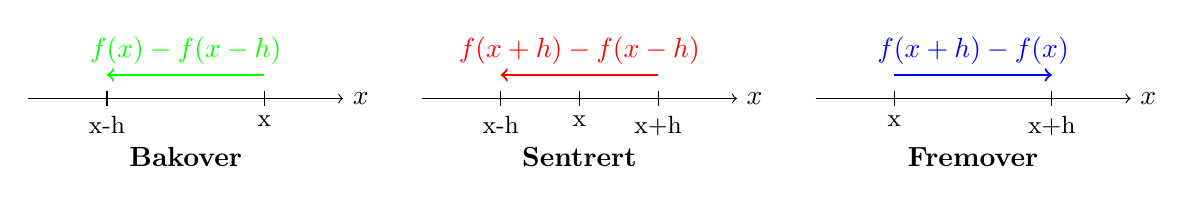
\begin{tikzpicture}
		% Backward Difference Scope
		\begin{scope}[xshift=-5cm]
			\draw[->] (-1,0) -- (3,0) node[right] {$x$}; % Number Line
			\foreach \x/\label in {0/$x-h$, 2/$x$} {
					\draw (\x,0.1) -- (\x,-0.1); % Points
					\node[below] at (\x,-0.1) {\small $\label$}; % Labels
				}
			\draw[->, thick, green] (2,0.3) -- (0,0.3) node[midway, above] {$f(x) - f(x-h)$}; % Arrow for difference
			\node[below] at (1, -0.5) {\textbf{Bakover}}; % Label
		\end{scope}

		% Central Difference Scope
		\begin{scope}[xshift=0cm]
			\draw[->] (-1,0) -- (3,0) node[right] {$x$};
			\foreach \x/\label in {0/$x-h$, 1/$x$, 2/$x+h$} {
					\draw (\x,0.1) -- (\x,-0.1); % Points
					\node[below] at (\x,-0.1) {\small $\label$};
				}
			\draw[->, thick, red] (2,0.3) -- (0,0.3) node[midway, above] {$f(x+h) - f(x-h)$};
			\node[below] at (1, -0.5) {\textbf{Sentrert}};
		\end{scope}

		% Forward Difference Scope
		\begin{scope}[xshift=5cm]
			\draw[->] (-1,0) -- (3,0) node[right] {$x$};
			\foreach \x/\label in {0/$x$, 2/$x+h$} {
					\draw (\x,0.1) -- (\x,-0.1);
					\node[below] at (\x,-0.1) {\small $\label$};
				}
			\draw[->, thick, blue] (0,0.3) -- (2,0.3) node[midway, above] {$f(x+h) - f(x)$};
			\node[below] at (1, -0.5) {\textbf{Fremover}};
		\end{scope}
	\end{tikzpicture}
	\caption{Finite Difference Stencils: Backward, Central, and Forward Difference}
	\label{fig:finite-differences}
\end{figure}


Som figuren viser, benytter \textbf{fremover}-differanser hovedsakelig punkter \emph{til høyre} for \(x_i\),
\textbf{bakover}-differanser benytter hovedsakelig punkter \emph{til venstre} for \(x_i\),
mens \textbf{sentrerte}-differanser er symmetriske rundt \(x_i\).


\section*{Endelig differanseskjema}

Endelige differanseformler gir diskrete tilnærminger av deriverte ved å bruke funksjonsverdier i strategisk utvalgte punkter (ofte kalt \emph{stencil}).
Kolonnene merket \(\mathbf{-3}\) til \(\mathbf{+3}\) (eller flere, avhengig av formelens bredde) oppgir \emph{dimensjonsløse koeffisienter} som multipliserer funksjonsverdiene i \(x_{i + k}\).

For å beregne den deriverte numerisk, må du så dividere med \(h^n\), der \(n\) er den deriverteordenen:

\[
	\frac{d^n f}{dx^n} \Bigg|_{x_i} \approx \frac{1}{h^n} \sum_{k=-m}^{m} \bigl( c_k f(x_{i+k}) \bigr)
\]

\begin{itemize}
	\item \(m\) er halvparten av stencilens bredde (f.eks. 3 for en 7-punkts stencil).
	\item \(c_k\) er dimensjonsløse koeffisienter.
\end{itemize}

\begin{table}[H]
	\centering
	\caption{Finite Difference Coefficients for Various Orders of Accuracy}
	\begin{tabular}{llrrrrrrrl}
		\toprule
		\multirow{2}{*}{Order} & \multirow{2}{*}{Type} & \multicolumn{7}{c}{Coefficients at Position} & \multirow{2}{*}{Error} \\
		\cmidrule{3-9}
		& & \textbf{-3} & \textbf{-2} & \textbf{-1} & \textbf{0} & \textbf{+1} & \textbf{+2} & \textbf{+3} & \\
		\midrule
		\multirow{3}{*}{First} & Forward & & & & -1 & 1 & & & $O(h)$ \\
		& Central & & & -1/2 & 0 & 1/2 & & & $O(h^2)$ \\
		& Backward & & & -1 & 1 & & & & $O(h)$ \\
		\midrule
		\multirow{3}{*}{Higher} & Forward & & & & -3/2 & 2 & -1/2 & & $O(h^2)$ \\
		& Central & & -1/12 & 2/3 & 0 & -2/3 & 1/12 & & $O(h^4)$ \\
		& Backward & & & 1/2 & -2 & 3/2 & & & $O(h^2)$ \\
		\midrule
		\multirow{3}{*}{Second} & Forward & & & & 1 & -2 & 1 & & $O(h^2)$ \\
		& Central & 1/12 & -2/3 & 0 & 2/3 & -1/12 & & & $O(h^4)$ \\
		& Backward & & & 1 & -2 & 1 & & & $O(h^2)$ \\
		\bottomrule
	\end{tabular}
	\label{tab:fd-coefficients}
\end{table}

\begin{example}{}{}
  Hvis vi ønsker å bruke en fremover differanseformel for den første deriverte med $O(h^3)$ nøyaktighet, kan vi bruke koeffisientene fra tabellen: \( \{-11, 18, -9, 2\} \).
  
  Dette gir oss:
  \begin{align*}
    \frac{d}{dx} f(x) & \approx \frac{1}{h} \left( -11f(x) + 18f(x+h) - 9f(x+2h) + 2f(x+3h) \right) \\
                     & = \frac{-11f(x) + 18f(x+h) - 9f(x+2h) + 2f(x+3h)}{h}
  \end{align*}

  For en fremover differanseformel av den andre deriverte med $O(h^2)$ nøyaktighet kan vi bruke koeffisientene: \(\{2, -5, 4, -1\}\).
  
  \medskip
  
  Dette gir oss:
  \begin{align*}
    \frac{d^2}{dx^2} f(x) & \approx \frac{1}{h^2} \left( 2f(x) - 5f(x+h) + 4f(x+2h) - f(x+3h) \right) \\
                         & = \frac{2f(x) - 5f(x+h) + 4f(x+2h) - f(x+3h)}{h^2}
  \end{align*}
\end{example}

\vspace{1em}

\noindent\textbf{Tips for bruk:}
\begin{itemize}
	\item Kontroller alltid \emph{tegnkonvensjon og indeksering} \(\;f(x_{i+k}) \leftrightarrow \text{koeffisient under kolonne }k\).
	\item Etter at koeffisientene er multiplisert med funksjonsverdiene, \emph{deler med} \(h^n\) for en \(n\)-te deriverte.
	\item Fremover/bakover brukes ofte nær kantene av et domene for å unngå ute-av-rekkevidde-punkter.
	\item Sentrerte differanser gir vanligvis høyere nøyaktighet enn fremover- eller bakoverdifferanser, siden de utnytter symmetrien rundt punktet ved å bruke naboverdier likt på begge sider.
\end{itemize}

\section{CFL-betingelsen (Courant-Friedrichs-Lewy)}

CFL-betingelsen er et nødvendig kriterium for stabilitet i tidsdiskretiseringer av hyperbolske og parabolske \gls{pde}. Betingelsen sikrer at det numeriske domenet av avhengighet inkluderer det fysiske domenet av avhengighet.

\begin{definition}{Courant-tall}{courant_number}
	Courant-tallet er definert som:
	\begin{equation}
		C = \frac{u \Delta t}{\Delta x}
	\end{equation}
	der $u$ er bølgehastigheten, $\Delta t$ er tidssteget, og $\Delta x$ er romsteget.
\end{definition}

\subsection{CFL-betingelser for ulike ligninger og skjemaer}

\begin{table}[H]
	\centering
	\caption{CFL-betingelser for ulike typer differensialligninger og numeriske skjemaer}
	\begin{tabular}{lllll}
		\toprule
		\textbf{Ligning} & \textbf{Skjema} & \textbf{CFL-betingelse} & \textbf{Kommentar} & \textbf{Stabilitet} \\
		\midrule
		\multirow{4}{*}{Adveksjon} & FTCS & $C \leq 1$ & $C = \frac{u\Delta t}{\Delta x}$ & Betinget stabil \\
		& Upwind (fremover) & $C \leq 1$ & $C = \frac{|u|\Delta t}{\Delta x}$ & Betinget stabil \\
		& Lax-Wendroff & $C \leq 1$ & $C = \frac{|u|\Delta t}{\Delta x}$ & Betinget stabil \\
		& Implisitt & Ingen & - & Ubetinget stabil \\
		\midrule
		\multirow{4}{*}{Diffusjon} & Eksplisitt & $r \leq \frac{1}{2}$ & $r = \frac{D\Delta t}{(\Delta x)^2}$ & Betinget stabil \\
		& Implisitt (BTCS) & Ingen & - & Ubetinget stabil \\
		& Crank-Nicolson & Ingen & - & Ubetinget stabil \\
		& DuFort-Frankel & $r < \frac{1}{2\mu}$ & $\mu = \sin^2\frac{\pi\Delta x}{\lambda_{min}}$ & Betinget stabil \\
		\midrule
		\multirow{3}{*}{Bølge} & Eksplisitt & $C \leq 1$ & $C = \frac{c\Delta t}{\Delta x}$ & Betinget stabil \\
		& Implisitt & Ingen & - & Ubetinget stabil \\
		& Leapfrog & $C \leq 1$ & $C = \frac{c\Delta t}{\Delta x}$ & Betinget stabil \\
		\midrule
		\multirow{3}{*}{Konveksjon-diffusjon} & Eksplisitt & $C \leq 1, r \leq \frac{1}{2}$ & Begge må oppfylles & Betinget stabil \\
		& FTCS & $r \leq \frac{1}{2}, P_e \leq 2$ & $P_e = \frac{|u|\Delta x}{D}$ & Betinget stabil \\
		& Upwind & $C \leq 1$ & - & Betinget stabil \\
		\midrule
		\multirow{2}{*}{2D Adveksjon} & Eksplisitt & $C_{2D} \leq 1$ & $C_{2D} = \Delta t \left( \frac{|u_x|}{\Delta x} + \frac{|u_y|}{\Delta y} \right)$ & Betinget stabil \\
		& Alternativt vilkår & $C_{alt} \leq 1$ & $C_{alt} = \Delta t \sqrt{ \frac{u_x^2}{\Delta x^2} + \frac{u_y^2}{\Delta y^2} }$ & Betinget stabil \\
		\midrule
		\multirow{2}{*}{2D Diffusjon} & Eksplisitt & $r_{2D} \leq \frac{1}{4}$ & $r_{2D} = D\Delta t \left( \frac{1}{(\Delta x)^2} + \frac{1}{(\Delta y)^2} \right)$ & Betinget stabil \\
		& Alternativt vilkår & $r_{alt} \leq \frac{1}{2d}$ & $d$ = antall dimensjoner & Betinget stabil \\
		\bottomrule
	\end{tabular}
	\label{tab:cfl-conditions}
\end{table}

\subsection{Fysisk tolkning av CFL-betingelsen}

\begin{itemize}
	\item $C < 1$: Informasjon reiser mindre enn én celle per tidssteg (sikker)
	\item $C = 1$: Informasjon reiser nøyaktig én celle per tidssteg (grensetilfelle)
	\item $C > 1$: Informasjon reiser mer enn én celle per tidssteg (ustabilt)
\end{itemize}

\begin{figure}[H]
	\centering
	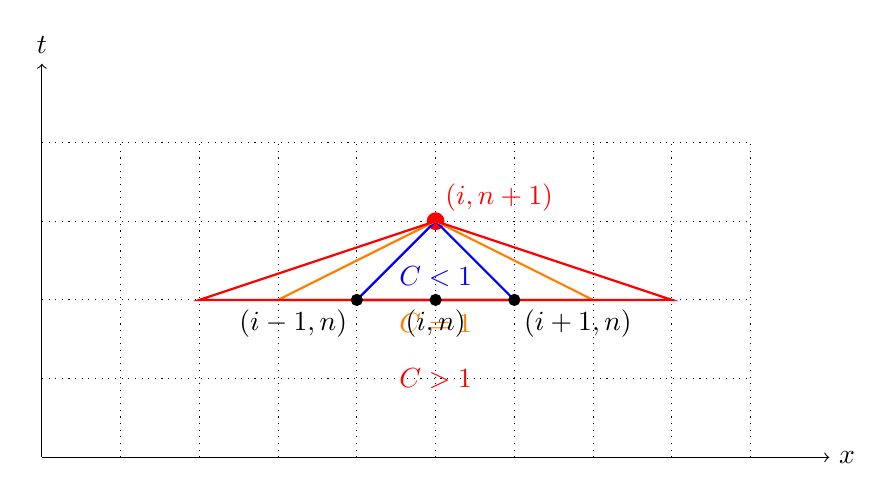
\begin{tikzpicture}
		% Tidsaksen
		\draw[->] (0,0) -- (10,0) node[right] {$x$};
		\draw[->] (0,0) -- (0,5) node[above] {$t$};
		
		% Rutenett
		\foreach \x in {1,2,...,9}
		\draw[dotted] (\x,0) -- (\x,4);
		\foreach \y in {1,2,...,4}
		\draw[dotted] (0,\y) -- (9,\y);
		
		% Punkt hvor vi beregner løsningen
		\filldraw[red] (5,3) circle (3pt);
		\node[red, above right] at (5,3) {$(i,n+1)$};
		
		% Domene av avhengighet i stabil situasjon (C < 1)
		\draw[blue, thick] (5,3) -- (4,2) -- (6,2) -- cycle;
		\node[blue] at (5,2.3) {$C < 1$};
		
		% Domene av avhengighet i grensetilfelle (C = 1)
		\draw[orange, thick] (5,3) -- (3,2) -- (7,2) -- cycle;
		\node[orange] at (5,1.7) {$C = 1$};
		
		% Domene av avhengighet i ustabil situasjon (C > 1)
		\draw[red, thick] (5,3) -- (2,2) -- (8,2) -- cycle;
		\node[red] at (5,1) {$C > 1$};
		
		% Punkter som brukes i beregningen
		\filldraw[black] (4,2) circle (2pt);
		\filldraw[black] (5,2) circle (2pt);
		\filldraw[black] (6,2) circle (2pt);
		\node[below left] at (4,2) {$(i-1,n)$};
		\node[below] at (5,2) {$(i,n)$};
		\node[below right] at (6,2) {$(i+1,n)$};
	\end{tikzpicture}
	\caption{Illustrasjon av CFL-betingelsen med numeriske og fysiske domener av avhengighet}
	\label{fig:cfl-condition}
\end{figure}

\subsection{Praktiske tilnærminger}

\begin{enumerate}
	\item \textbf{Adaptivt tidssteg:} Beregn tillatt $\Delta t$ for hvert steg basert på gjeldende $\Delta x$ og fysiske parametre.
	
	\item \textbf{Global reduksjon:} Multipliser teoretisk maksimum $\Delta t$ med en sikkerhetsfaktor (typisk $0.8-0.9$).
	
	\item \textbf{Alternative metoder:} Vurder implisitte metoder for problemer med strenge CFL-betingelser.
\end{enumerate}

\begin{example}{Beregning av maksimalt tidssteg}{cfl_example}
	For en adveksjonsligning med $u = 100$ m/s og $\Delta x = 0.01$ m:
	\begin{align*}
		\Delta t &\leq \frac{\Delta x}{|u|} \\
		\Delta t &\leq \frac{0.01}{100} = 0.0001 \text{ s}
	\end{align*}
	Med en sikkerhetsfaktor på $0.9$ vil det praktiske tidssteget bli $\Delta t = 9 \times 10^{-5}$ s.
\end{example}

